\begin{figure}[h!]
\begin{center}
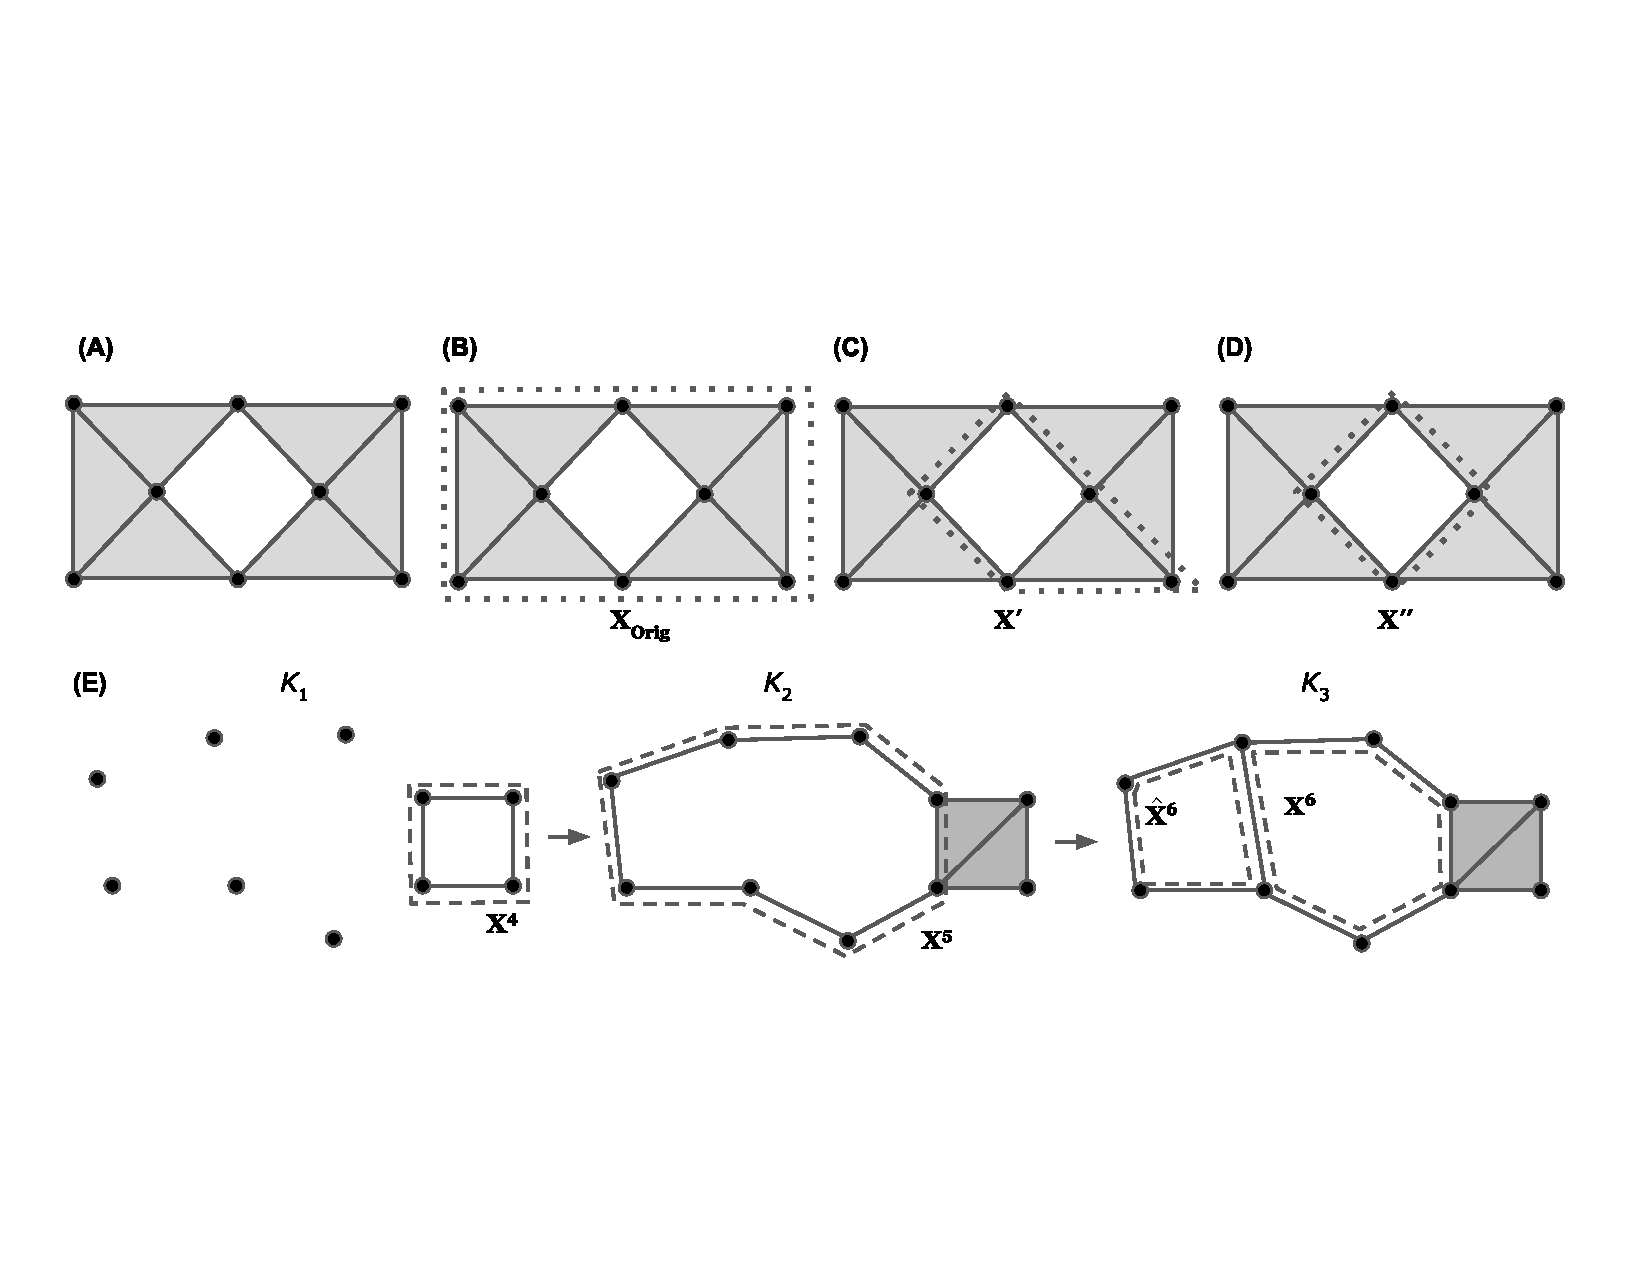
\includegraphics[width=1\textwidth]{figures/examplesminimal.pdf}% This is a *.eps file
\end{center}
\caption{Examples of optimizing a cycle representative (using the notion of minimizing edges) within the same homology class (\textbf{A-D}) and using a basis of cycle representatives (\textbf{E}), modified examples taken from \cite{Escolar2016} and \cite{Obayashi2018}. The dotted lines represent a cycle representative for the enclosed ``hole''. Intuitively, we consider $\optimalrep''$ in (\textbf{D}) as the optimal cycle representative since it consists of the smallest number of edges. Subfigure (\textbf{E}) shows a case where we optimize a cycle representative using a basis of cycle representatives. In (\textbf{E}), $\{\optimalrep^4, \optimalrep^5, \optimalrep^6\}$ is the original basis of cycle representatives. We can substitute $\optimalrep^6$ with $\hat{\optimalrep}^6$, which we can obtain by adding $\optimalrep^5$ to $\optimalrep^6$, and thus obtain $\{\optimalrep^4, \optimalrep^5, \hat{\optimalrep}^6\}$ as the new basis of cycle representatives.}\label{fig:example-optimal}
\end{figure}
